
\section{Machine Learning}

Sono state implementate diverse tecniche: K-Nearest-Neighbors e Recurrent Neural Networks (Long Short-Term Memory e Gated Recurrent Network)



% -----------------------------------------------------


\subsection{KNN}

L'algoritmo prevede i valori futuri basandosi sui k Nearest Neighbors. Viene utilizzata una metodologia MIMO (multi-input multi-output). 

Per la scelta dei valori degli iperparametri k (numero di osservazioni passate da considerare) e p (quante sottosequenze simili guardare) è stata effettuata una serie di test, andando a prendere quelli che minimizzassero il MAPE sul validation set. I valori testati sono: k in [4, 8, 16, 32, 64] e p in [12, 24, 24*2, 24*4, 24*7, 24*14, 24*21, 24*28]. Si sarebbe potuta effettuare una grid-search più intensa, ma è stato preferito in questo modo al fine di avere una maggiore interpretabilità e velocità di esecuzione. Inoltre, usare la mediana ha fornito risultati leggermente migliori della media. 

I migliori risultano essere $k=8$ e $p = 504$ (tre settimane), ottenendo un MAPE di 10.13\%.

\begin{figure}[H]
\centering
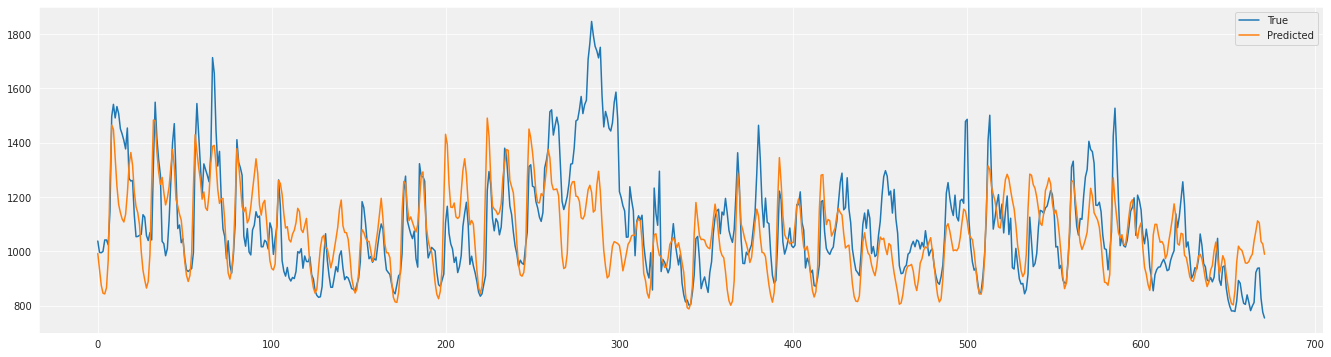
\includegraphics[width=14cm]{Pictures/prediction_knn.png}
\caption{Previsione finale del KNN.}
\end{figure}



% -----------------------------------------------------


\subsection{LSTM}

Per prima cosa, i dati sono stati sottoposti a del preprocessing: oltre ad una normalizzazione tra 0 e 1 (ovviamente rispetto al training set), hanno subito un reshape per essere dati in input alla rete. In particolare, è stata scelta una previsione recursive multi-step, predicendo una settimana alla volta. Questa tecnica fornisce risultati migliori rispetto ad una single-step o ad una multi-step giornaliera. La finestra ottimale sui dati precedenti è di tre settimane.

Sono state effettuate inoltre diverse prove sulla struttura del modello. Il migliore, che cerca di non essere troppo complesso per un trade-off sul tempo di allenamento (i modelli lineari sono estremamente più veloci), è così costruito: 
\begin{itemize}
    \item LSTM di 512 unità, con funzione di attivazione ReLU
    \item Dropout di 0.1
    \item LSTM di 256 unità, con funzione di attivazione ReLU
    \item Dropout di 0.1
    \item Dense di 168 unità (per predizione valori della settimana successiva)
\end{itemize}

Per quanto riguarda il numero di epoche, è stato effettuato un early stopping con patience=3, su 100 epoche, con un batch size di 128 osservazioni.

La previsione avviene settimana per settimana: prendendo in input l'ultimo mese del training set, predice una settimana; aggiorna poi i dati prendendo tre settimane del training set e quella predetta; così via fino ad arrivare ad un mese. Il modello con il MAPE minore risulta essere 10.43\%.

\begin{figure}[H]
\centering
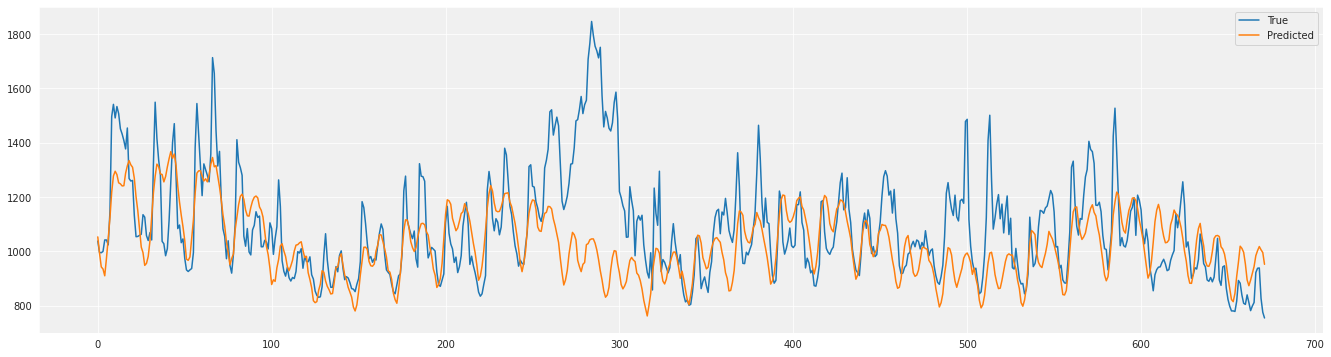
\includegraphics[width=14cm]{Pictures/prediction_lstm.png}
\caption{Previsione finale della RNN con LSTM.}
\end{figure}


% -----------------------------------------------------


\subsection{GRU}

Per le GRU, i dati subiscono lo stesso preprocessing delle LSTM. Anche la struttura della rete viene mantenuta, sostituendo però i layer LSTM con dei layer GRU. Il procedimento è lo stesso in tutto e per tutto, in quanto sembra essere la migliore impostazione anche per questo tipo di RNN. Il modello ottiene un MAPE di 10.93\%

\begin{figure}[H]
\centering
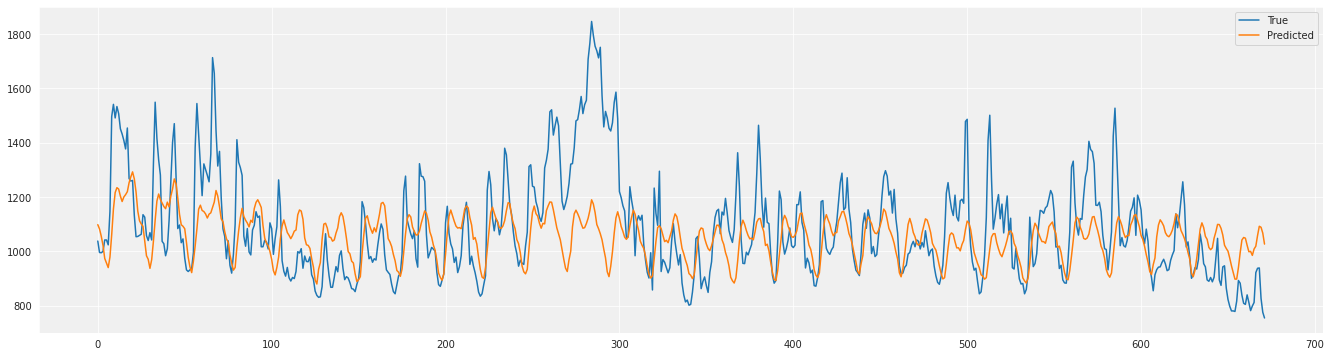
\includegraphics[width=14cm]{Pictures/prediction_gru.png}
\caption{Previsione finale della RNN con GRU.}
\end{figure}


